\documentclass{article}
\usepackage[utf8]{inputenc}

\title{NTIN066 - Hash}
\author{Thuong-Hai Pham}
\date{December 2017}

\usepackage{natbib}
\usepackage{graphicx}

\begin{document}

\maketitle

\section{Random case}

In Random case study, 50 experiments were executed. Each experiment stopped when load factor is larger than 0.99 (linear probing) or the number of rehashing operations (cuckoo hashing) exceeds 20 (which equals to the log size of hash table).

\begin{figure}[h!]
\centering
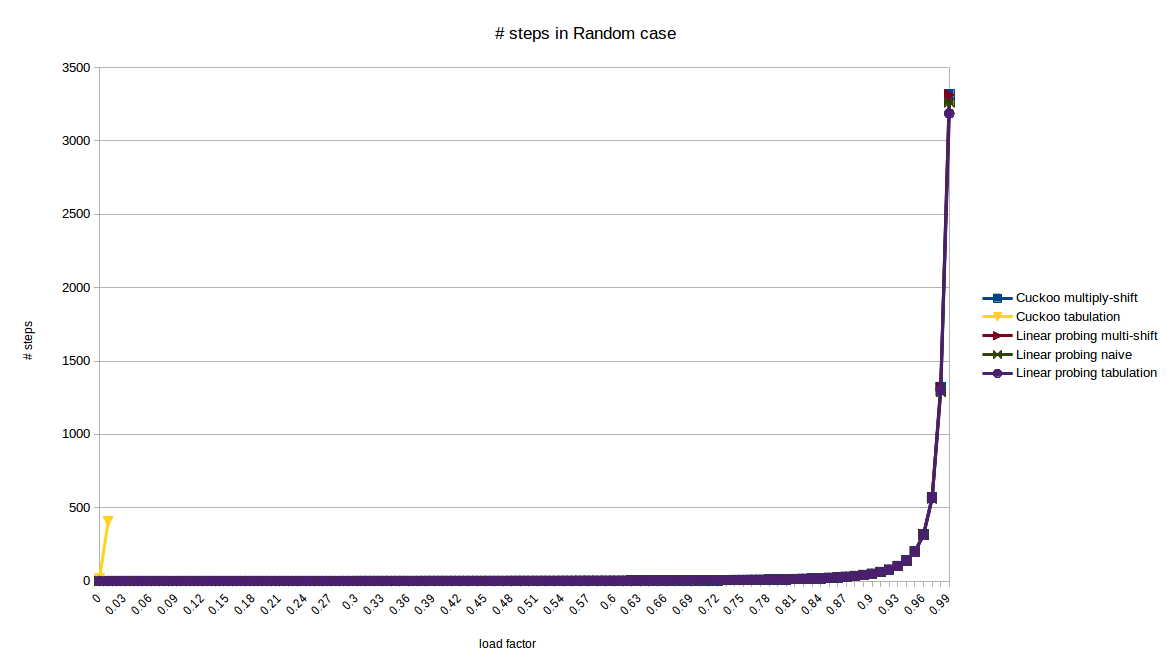
\includegraphics[width=\textwidth]{0_steps.png}
\caption{Average number of steps of Insert operation}
\label{fig:0_steps}
\end{figure}

\begin{figure}[h!]
\centering
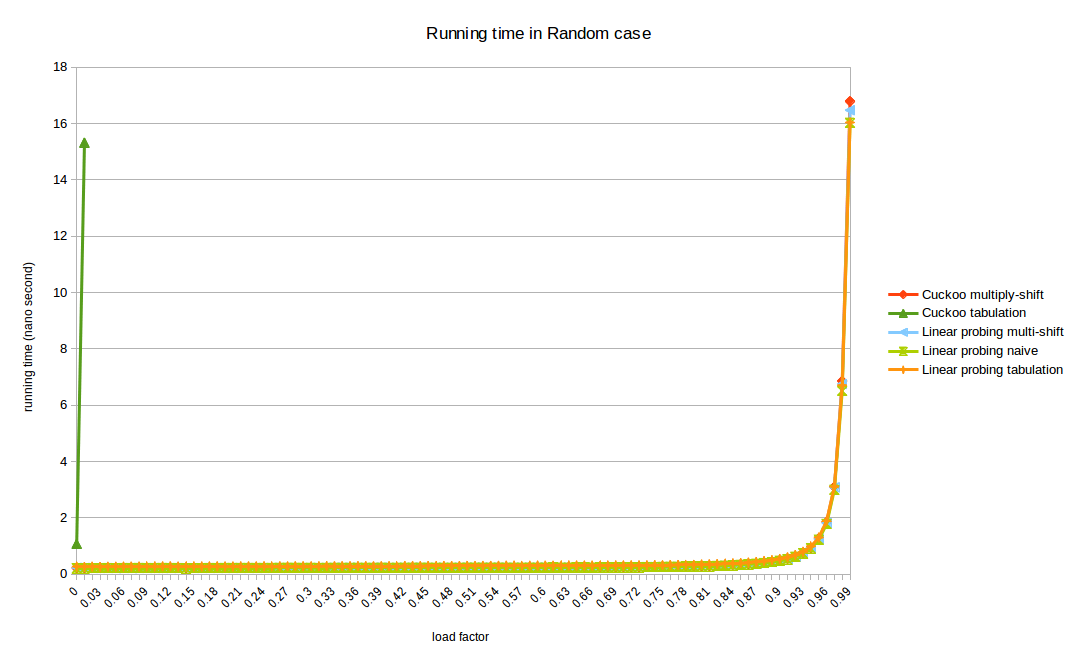
\includegraphics[width=\textwidth]{0_time.png}
\caption{Average running time of Insert operation}
\label{fig:0_time}
\end{figure}

Figure \ref{fig:0_steps} and \ref{fig:0_time} show the results in Random case study. It is clearly that both the average number of steps and average running time of Insert operation in most of the combinations grow exponentially, except ``Cuckoo hashing with tabulation" (Cuckoo-tab). The results of Cuckoo-tab from load factor of 0.02 have been removed from the graph for readability as they grow extremely fast (average number of steps at 0.02 is 22582.304981, and which average running time is 840.996119 nano seconds). This behavior can be explained by the fact that Cuckoo-tab use two tabulation hash function. These functions are implemented to retry as many time as the size of the hash table before rehashing instead of detecting if a cycle exists. Hence, that lead to a significantly higher number of steps (swap operations) in tabulation.

\section{Sequential inserts into a table using linear probing}
In this case study, for every value of m, 50 experiments were executed.

\begin{figure}[h!]
\centering
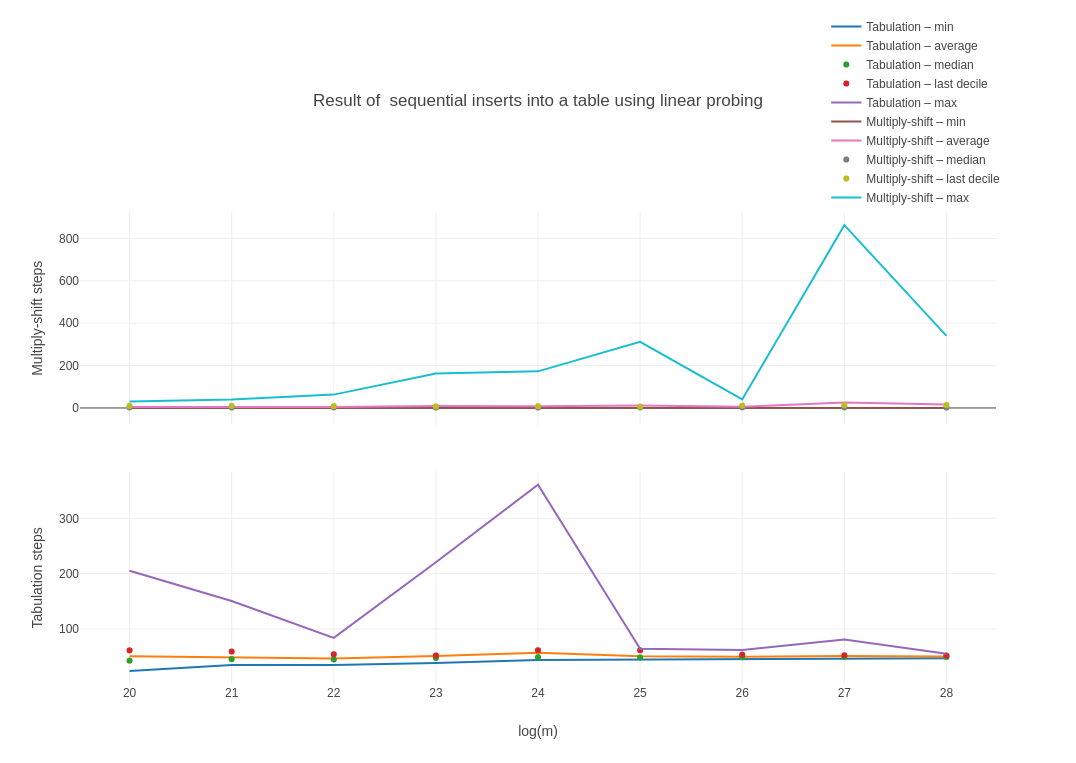
\includegraphics[width=\textwidth]{1.png}
\caption{Sequential inserts into a table using linear probing result}
\label{fig:plot2}
\end{figure}

From Figure \ref{fig:plot2}, linear probing with multiply-shift hash function has a better result than tabulation as most of the values from minimum to last decile fluctuate from 0 to 25.47. While in tabulation, these values are ranging from 24.12 to 61.28. Figure \ref{fig:plot2b} clearly illustrates this observation by leaving the minimum and maximum lines out, which are affected by the small number of experiments.

\begin{figure}[h!]
\centering
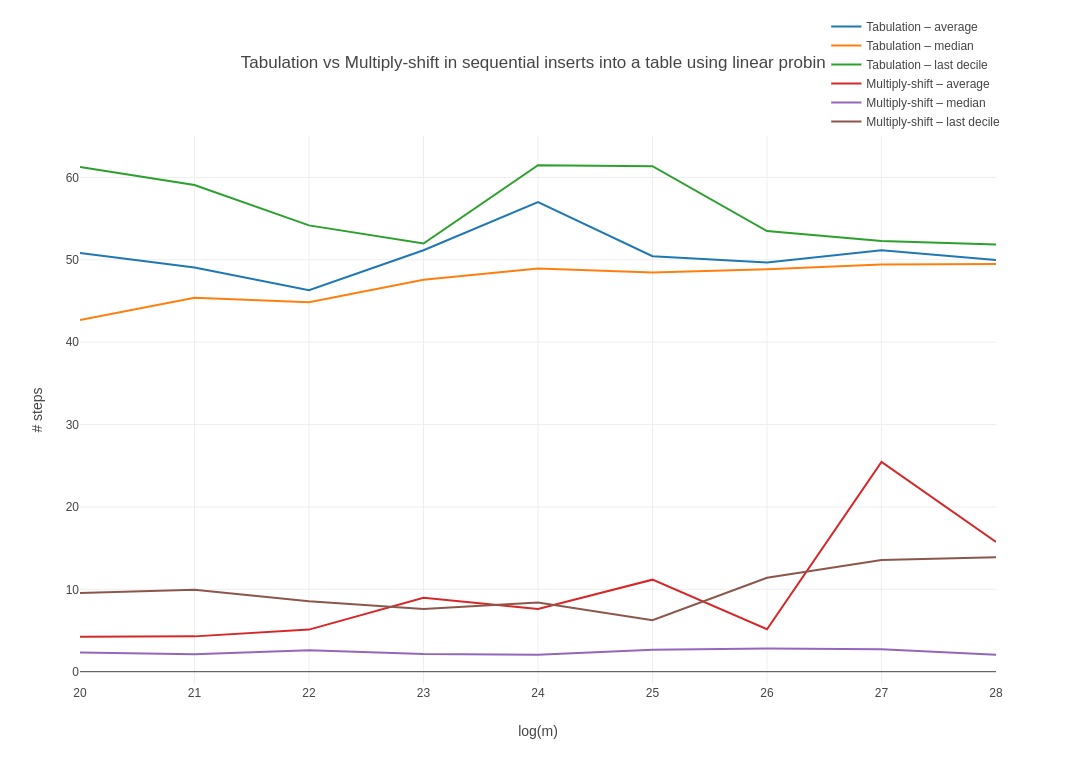
\includegraphics[width=\textwidth]{1b.png}
\caption{Sequential inserts into a table using linear probing result (without min and max)}
\label{fig:plot2b}
\end{figure}


\end{document}
